\section{Rediseño de FuD}


\begin{frame}\frametitle{Rediseño de FuD}	
	\begin{block}{}
		Durante el desarrollo de este proyecto se debieron efectuar diversos cambios en el diseño e implementación 
		original de FuD para poder integrar esta nueva capa de distribución.
	\end{block}
	\vspace{4mm}
	\begin{itemize}\addtolength{\itemsep}{4mm}
		\item Redeclaración del método \texttt{create\_distribution\_client()}
		\item \texttt{JobManager} post initialization
		\item Reenvío de \texttt{JobUnits} configurable
		\item Múltiples \texttt{JobUnits} a clientes
	\end{itemize}
\end{frame}


\begin{subsection}{Redeclaración del método \texttt{create\_distribution\_client()}}

	\begin{frame}[fragile]\frametitle{Redeclaración del método \texttt{create\_distribution\_client()}}	
		\begin{block}{}
			Método provisto por \fud \ para la creación de un cliente de distribución.
		\end{block}
		\vspace{4mm}
		Prototipo original:
		\begin{lstlisting}
		DistributionClient* create_distribution_client(
		        std::string address = "127.0.0.1", Port port = 31337);
		\end{lstlisting}
		\vspace{4mm}		
		Prototipo actual:
		\begin{lstlisting}
		DistributionClient* create_distribution_client(
		        int argc, char** argv);
   		\end{lstlisting}
	\end{frame}

\end{subsection}


\begin{subsection}{\texttt{JobManager} post initialization}

	\begin{frame}[fragile]\frametitle{\texttt{JobManager} post initialization}
  		\begin{figure}[h] 		
    		\begin{minipage}{0.26 \textwidth}
      			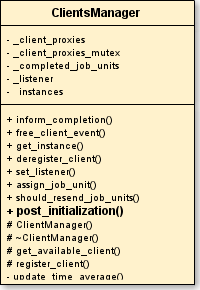
\includegraphics[scale=0.5]{images/ClientsManager-post-init.png}
    		\end{minipage}
    		\hfill
    		\begin{minipage}{0.64 \textwidth}
      			\begin{block}{}
      				\begin{itemize}\addtolength{\itemsep}{6mm}
						\item Se agregó un nuevo método en la clase \texttt{ClientsManager} de \fud.
						\item Por defecto, su implementación es vacía.
						\item El método sólo es invocado al final del constructor de \texttt{JobManager}:
						\begin{lstlisting}
							_clients_manager->post_initialization()
						\end{lstlisting}
					\end{itemize}
      			\end{block}
      		\end{minipage}
      	\end{figure}
	\end{frame}
	
	\begin{frame}[fragile]\frametitle{Redefinición de \texttt{post\_initialization()}}
		\begin{block}{Declaración y definición en \texttt{ClientsManager}}
			\begin{lstlisting}
				virtual void post_initialization() {};
			\end{lstlisting}
		\end{block}
		
		\begin{block}{Redefinición en \texttt{BoincClientsManager}}
			\begin{lstlisting}
				void BoincClientsManager::post_initialization()
				{    boinc_register_client();    }
			\end{lstlisting}
			\begin{lstlisting}
				void BoincClientsManager::boinc_register_client()
				{
				    // Init the client_proxy.
				    boinc_log_debug(std::string("Registering BOINC with FuD."));
				    BoincClientProxy * client = new BoincClientProxy();
				    client->set_concurrent_jobs(UNLIMITED_JOBS);
				    // Register the unique client proxy.
				    register_client(client);
				}
			\end{lstlisting}
		\end{block}
	\end{frame}

\end{subsection}


\begin{subsection}{Reenvío de \texttt{JobUnits} configurable}

	\begin{frame}[fragile]\frametitle{Reenvío de \texttt{JobUnits} configurable}
  		\begin{figure}[h] 		
    		\begin{minipage}{0.26 \textwidth}
      			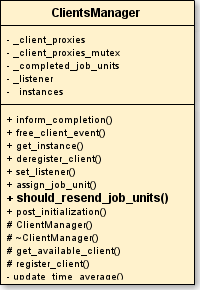
\includegraphics[scale=0.5]{images/ClientsManager-resend-jobunit.png}
    		\end{minipage}
    		\hfill
    		\begin{minipage}{0.64 \textwidth}
      			\begin{block}{}
      				\begin{itemize}\addtolength{\itemsep}{4mm}
						\item Se agregó un nuevo método en la clase \texttt{ClientsManager} de \fud.
							\begin{lstlisting}[basicstyle=\tiny]
								virtual bool should_resend_job_units() = 0;
							\end{lstlisting}
						\item Definición del método en \texttt{BoincClientsManager}:
							\begin{lstlisting}[basicstyle=\tiny]
								bool BoincClientsManager::should_resend_job_units()
								{
								    return false;
								}
							\end{lstlisting}
					\end{itemize}
      			\end{block}
      		\end{minipage}
      	\end{figure}
	\end{frame}
	
	\begin{frame}[fragile]\frametitle{Reimplementación de \texttt{handle\_free\_client\_event()}}
  		\begin{lstlisting}[basicstyle=\tiny, numbers=left, firstnumber=170]
	if (_jobQueue.empty())
	{
	    if (_clients_manager->should_resend_job_units()) 
	    {
	        if (! _pendingList.empty())
	        {
	            if (_clients_manager->assign_job_unit(*_pendingList.front()))
	            {
	                //send this one to the back, act as Round Robin
	                _pendingList.push_back(_pendingList.front());
	                _pendingList.pop_front();
	            }
	            else
	                syslog(LOG_NOTICE, "Error sending JobUnit %u from Pending List to a client.", _pendingList.front()->get_id());
	        }
	    }
	}
	else
	{
	    if (_clients_manager->assign_job_unit(*_jobQueue.front()))
	    {
	        syslog(LOG_NOTICE, "Sending JobUnit %u to pending list.", (_jobQueue.front()->get_id()));
	        _pendingList.push_back(_jobQueue.front());
	        _jobQueue.pop_front();
	    }
	    else
	        syslog(LOG_NOTICE, "Error sending JobUnit %u from Job Queue to a client.", _jobQueue.front()->get_id());
	}	
  		\end{lstlisting}
	\end{frame}
	
\end{subsection}


\begin{subsection}{Múltiples \texttt{JobUnits} a clientes}

	\begin{frame}\frametitle{Múltiples \texttt{JobUnits} a clientes}
		\begin{block}{Problema}
			Los clientes sólo pueden procesar a lo sumo de a una JobUnit por vez.
		\end{block}
		\pause
		\begin{block}{Solución}
			La idea general consiste en:
			\begin{enumerate}\addtolength{\itemsep}{2mm}
				\item Permitir configurar la cantidad máxima de tareas en simultáneo que un cliente puede ejecutar. \pause
				\item Llevar un registro de la cantidad de tareas que un cliente se encuentra computando en un determinado momento.\pause
				\item Determinar la disponibilidad de un cliente.\pause
				\item Si el cliente se encuentra disponible, generar un nuevo evento de cliente libre.
			\end{enumerate}
		\end{block}
	\end{frame}

	\begin{frame}\frametitle{ClientProxy}
		\begin{figure}
      		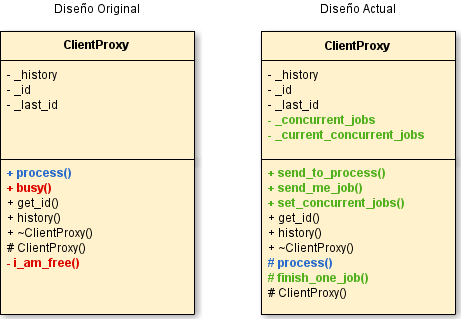
\includegraphics[scale=0.5]{images/ClientProxy-orig-vs-actual.png}
      	\end{figure}
	\end{frame}

	\begin{frame}\frametitle{ClientsManager}
		\begin{figure}
      		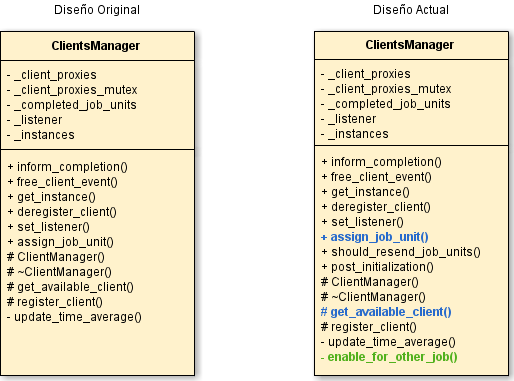
\includegraphics[scale=0.5]{images/ClientsManager-orig-vs-actual.png}
      	\end{figure}
	\end{frame}

	\begin{frame}\frametitle{Diagrama de secuencia: multiple jobs}
		\begin{figure}
      		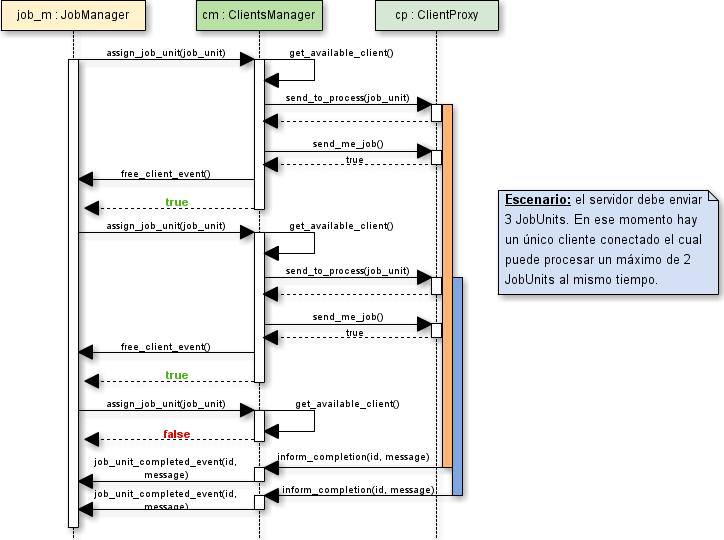
\includegraphics[scale=0.38]{images/diagr-sec-rediseno-mult-jobs.png}
      	\end{figure}
	\end{frame}



\end{subsection}
